\chapter{PAPER-128}
\label{c.PSA128}

\section{Overview}

The PAPER experiment expanded out to 128 antennas in 2013 and observed for two seasons. The first season began in November, 2013 and lasted until March, 2014. The second began in July, 2014 and ended in January, 2015. The PAPER-128 configuration consists of 112 core antennas arranged in a grid layout (7 rows and 16 columns), with neighboring East/West spacings being 15\,m and neighboring North/South spacings being 4\,m (Figure \ref{fig:paper128_array}). Additionally, 16 outrigger antennas were placed in strategic locations in order to form long baselines and increase \textit{uv}-plane sampling. These outrigger antennas are not used for the power spectrum analysis presented in this thesis, but are useful for imaging analyses.

\begin{figure}
	\centering
	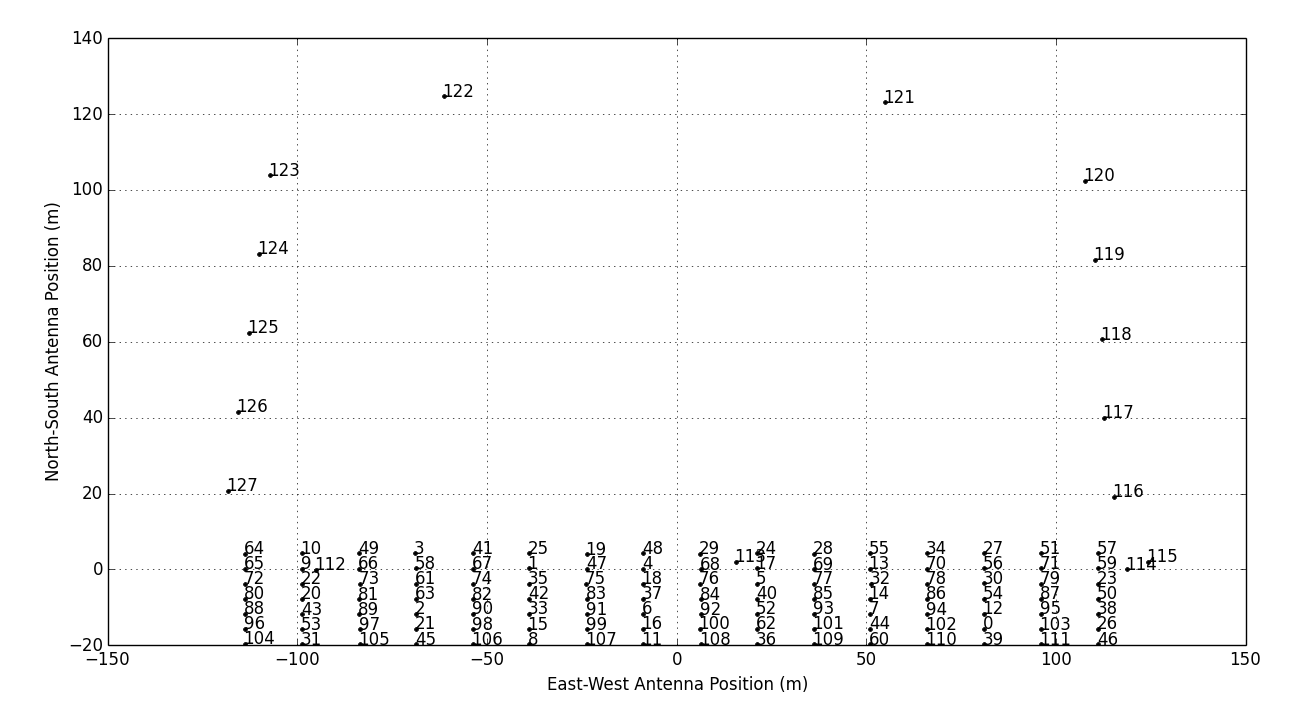
\includegraphics[width=0.96\textwidth]{plots/paper128_layout.png}
	\caption{The PAPER-128 antenna layout. There are 112 antennas arranged in a grid layout which are used for power spectrum analyses. The addition of 16 outrigger antennas is used to increase \textit{uv}-plane sampling for imaging analyses.}
	\label{fig:paper128_array}
\end{figure}

In general, the signal chain of PAPER-128 is similar to that of PAPER-64. However, one major change is the addition of receiverators on site, which houses the receivers used to amplify and filter the antenna signals. Prior to this change, the receivers were located inside a cooled shipping container along with the rest of the DSP system. With the addition of more antennas, however, the receivers were moved outside the container to save space. 

Although PAPER-128 doubled in number of antennas, the data collected by this array is typically found to be lower in quality than that of PAPER-64. There are many reasons for this, including general wear and tear on the instrument and the addition of the receiverators (which had no monitoring system and, as we will see, is one of the main reasons for missing and corrupted PAPER-128 data). Because of these issues, PAPER-128 requires the development of novel techniques in order to filter out contaminated data products prior to analysis. Using the entire season of data, without any filtering, would result in a power spectrum analysis severely dominated by systematics and (non-EoR) detections. Thus, one of the unique challenges facing PAPER-128 is how to automatically and accurately detect and remove bad data (i.e., misbehaving baselines, dead receiverators, criss-crossed signal paths, etc.) in order to curate a dataset as free of systematics as possible.

In this chapter, we present methods developed for the detection of corrupt data in PAPER-128. These methods represent the first routinely-used ``quality assurance" steps for the PAPER experiment. They also represent the first generation of data assessment techniques that are currently being expanded upon for incorporation into HERA's real-time processing system. 

\begin{table}[]
\begin{tabular}{|c|c|c|c|c|}
\hline
\textbf{Epoch} & \textbf{Dates}        & \textbf{\begin{tabular}[c]{@{}c@{}}Number of \\ Days Analyzed\end{tabular}} & \textbf{Flagged Days}                                                    & \textbf{Flagged Antennas}                                                                                                                         \\ \hline
1              & \begin{tabular}[c]{@{}c@{}} Nov 2013 - Jan 2014 \\ JDs 6617-6673\end{tabular}   & 38                                                                          & \begin{tabular}[c]{@{}c@{}}6647,6662,6664,\\ 6665,6673\end{tabular}      & \begin{tabular}[c]{@{}c@{}}3,7,8,16,19,20,\\ 27,28,34,53,\\ 56,84,85,96,100\\ \textbf{FX2}: 2,10,15,22,31,\\ 33,42,43,47,58,\\ 64,72,91,97,105,107\end{tabular} \\ \hline
2              & \begin{tabular}[c]{@{}c@{}} Jan 2014 - March 2014 \\JDs 6678-6724\end{tabular} & 40                                                                          & \begin{tabular}[c]{@{}c@{}}6692,6702,6704,\\ 6706,6717,6730\end{tabular} & \begin{tabular}[c]{@{}c@{}}3,7,16,27,34,56,\\57,84,85,100,110\end{tabular}                                                               \\ \hline
\end{tabular}
\caption{An overview of the PAPER-128 data used for power spectrum analysis in this thesis.}
\label{table:psa128_overview}
\end{table}

Additionally in this chapter, we process two epochs of PAPER-128 data (both from the first season) and show power spectrum results for each. We do not show results from the second season of data due to increased hardware failure that was experienced at the end of PAPER-128's deployment. As such, the first season of PAPER-128 represents the bulk of the array's sensitivity (though we note that the limits do not surpass those of PAPER-64, mostly due to having fewer days of data). Table \ref{table:psa128_overview} gives an overview of the PAPER-128 dataset analyzed in this thesis.

\section{Quality Assurance}

Post-processing of PAPER data relies heavily on the array's redundancy, and any sources of non-redundancy have the potential to corrupt redundant calibration and power spectrum estimation. These sources of error --- which span from the failure of analog or digital components to improper feed installation to the accidental deletion and subsequent recovery of data products --- manifest themselves in corrupted data that can be found primarily along two main axes: the time-axis and the antenna-axis. 

We next present metrics that we have developed to locate contaminated data along these axes. We use the results of these metrics to remove specific days of data and specific antennas from our analysis prior to calibration in order to ensure robust calibration that is not influenced by outlier data.

\subsection{Flagging Julian Dates}

To better assess the variation of PAPER-128 data across its two-year deployment (which consists of 7+ individual epochs of data, where an epoch is characterized by the shut-down and subsequent re-starting of the correlator), we first investigate one-dimensional slices of compressed data that span the entire time axis but only one frequency channel. We choose channel 100 for this analysis, as its corresponding frequency of 150\,MHz lies in the middle of our band (similar to PAPER-64, PAPER-128's bandwidth consists of 203 frequency channels ranging from 100 to 200\,MHz).

We look at the visibility amplitude of each day of data in an epoch as a function of LST, shown as the different colors in Figure \ref{fig:psa128_meanVij}. We designate a reference day to each epoch (a manually chosen ``good" day), and flag days that differ from the reference day by more than 20\%. After flagging, visibilities show good day-to-day agreement across an epoch (bottom row of Figure \ref{fig:psa128_meanVij}.

An example of data from a particularly ``bad" day is shown in Figure \ref{fig:psa128_badday}. It is clear that Julian date 2456692 differs dramatically from reference day 2456680, as it contains many corrupted files throughout the day due to failure somewhere in the signal chain. This failure mode is often due to the accidental deletion and erroneous recovery of data (much of the season's data was accidentally deleted prior to any of the work in this thesis), as well as hardware failures (e.g., loose cable connections) that result in lost sky fringes. From Table \ref{table:psa128_overview}, we see that a total of 38 days pass our flagging metric for Epoch 1 and 40 days pass for Epoch 2 (both from PAPER-128's first observing season), and a total of five and six days are flagged for each epoch, respectively.

\begin{figure*}
	\centering
	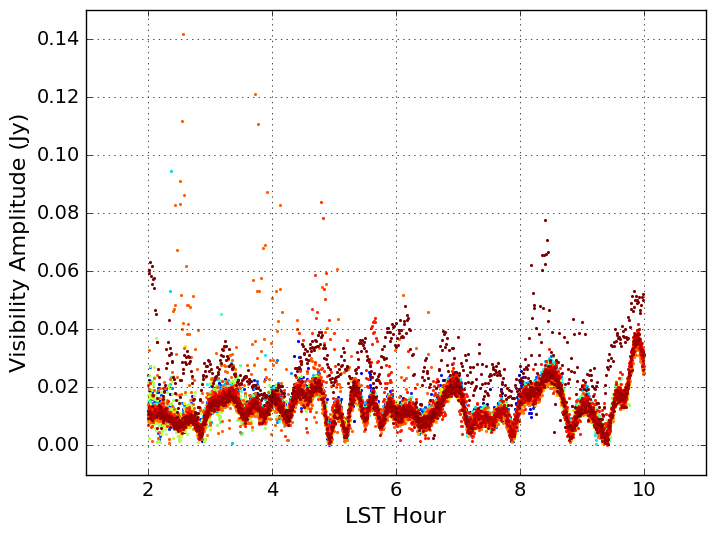
\includegraphics[trim={0cm 0cm 0cm 0cm},clip,height=0.35\textwidth]{plots/psa128_meanVij_S1E1_before.png}
	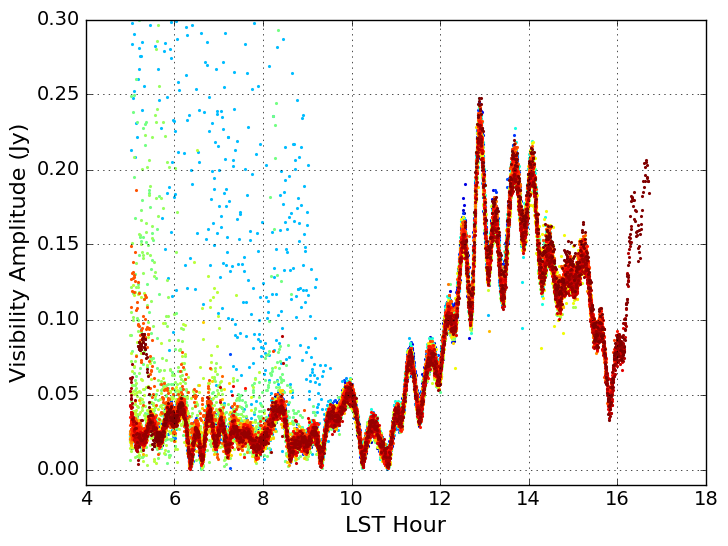
\includegraphics[trim={0cm 0cm 0cm 0cm},clip,height=0.35\textwidth]{plots/psa128_meanVij_S1E2_before.png}
	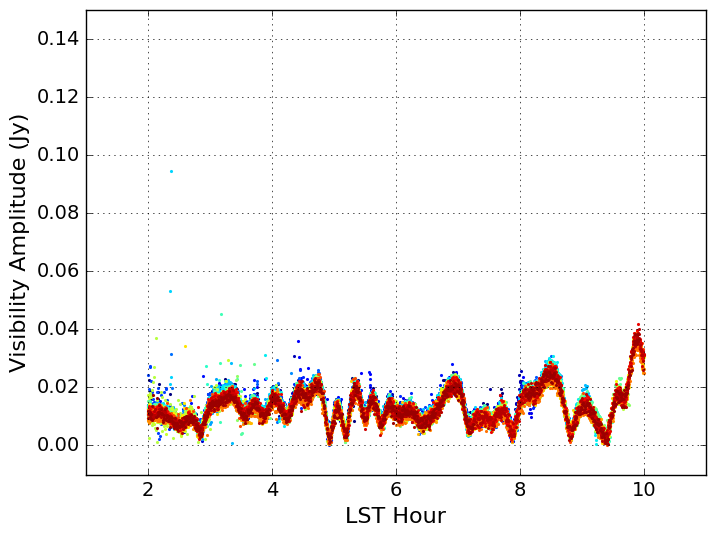
\includegraphics[trim={0cm 0cm 0cm 0cm},clip,height=0.35\textwidth]{plots/psa128_meanVij_S1E1_after.png}
	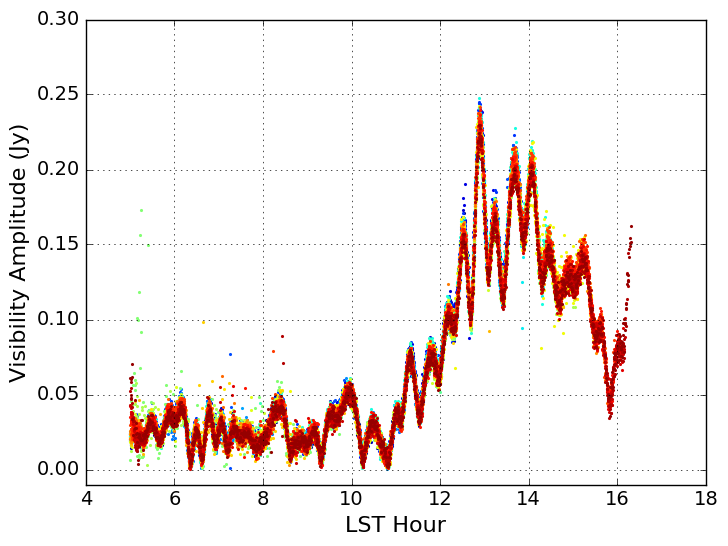
\includegraphics[trim={0cm 0cm 0cm 0cm},clip,height=0.35\textwidth]{plots/psa128_meanVij_S1E2_after.png}
	\caption{Visibility amplitudes as a function of LST for different Julian days of data (colors). The left column shows the data before (top) and after (bottom) the flagging of outlier days for Epoch 1. The right column shows similar data for Epoch 2. After flagging, visibilities show good day-to-day agreement across an epoch.}
	\label{fig:psa128_meanVij}
\end{figure*}

\begin{figure}
	\centering
	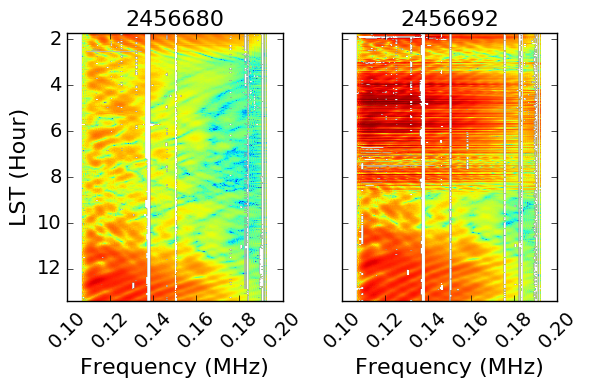
\includegraphics[width=0.8\textwidth]{plots/psa128_badday.png}
	\caption{Waterfall plots of visibility amplitudes for a ``good" reference day (left) in Epoch 2 and ``bad" day (right). We exclude corrupted data for specific days found with our metric.}
	\label{fig:psa128_badday}
\end{figure}

\subsection{Flagging Antennas}
\label{sec:psa128_badant}

There are a few types of failure modes for data associated with specific antennae. The first is if feeds are accidentally rotated by 90 degrees (or equivalently, the cables for the XX and YY polarizations are swapped). Consequently, visibilities involving a ``cross-polarized" antenna exhibit visibility amplitudes that are more weakly correlated (lower amplitude) than what is expected for an XX or YY visibility (and similarly, XY and YX visibilities exhibit too high of an amplitude, or too strong of a correlation). In order to locate potentially cross-polarized antennas, we use the following metric:

\begin{equation}
\label{eq:psa128_badant}
M_{i} = \frac{\sum\limits_{j,\nu,t} |V_{ij}|}{(N-1)},
\end{equation}
where the visibility for baseline $ij$ is summed for every $j^{th}$ antenna, frequency $\nu$, and time $t$, and $N$ is the number of antennas. We compute this metric for all four polarizations (XX, XY, YX, YY). Next, for each night of data we form the polarization fraction quantity:

\begin{equation}
\label{eq:psa128_crosspol}
P_{i} = \frac{M_{i}^{XY} + M_{i}^{YX}}{M_{i}^{XX} + M_{i}^{YY}}.
\end{equation}
We expect the numerator of this quantity to be higher than the denominator for cross-polarized antennae. In practice, we form polarization fractions for every antenna and flag those with high $P_{i}$ values as being cross-polarized. We note that this metric works best for long baselines, where XX and XY visibilities are expected to have large differences in signal-to-noise over short distance scales. For short baselines (and large-scales), astrophysical polarization has been shown to be present in all polarization quantities, including the linear ones, thus bringing $P_{i}$ closer to unity (\citealt{lenc_et_al2016}).

Using this metric, we find six antennas to be cross-polarized in PAPER-128 observations (antennas 26, 34, 38, 46, 50, and 72). An example of visibilities containing antenna 26 is shown in Figure \ref{fig:psa128_crosspol}, and it is clear that the ``X" and ``Y" polarizations are swapped for baselines involving that antenna. We fix this issue, re-naming polarization states where necessary, for all the compressed PAPER-128 data before performing other quality assessment tests and calibration.

\begin{figure}
	\centering
	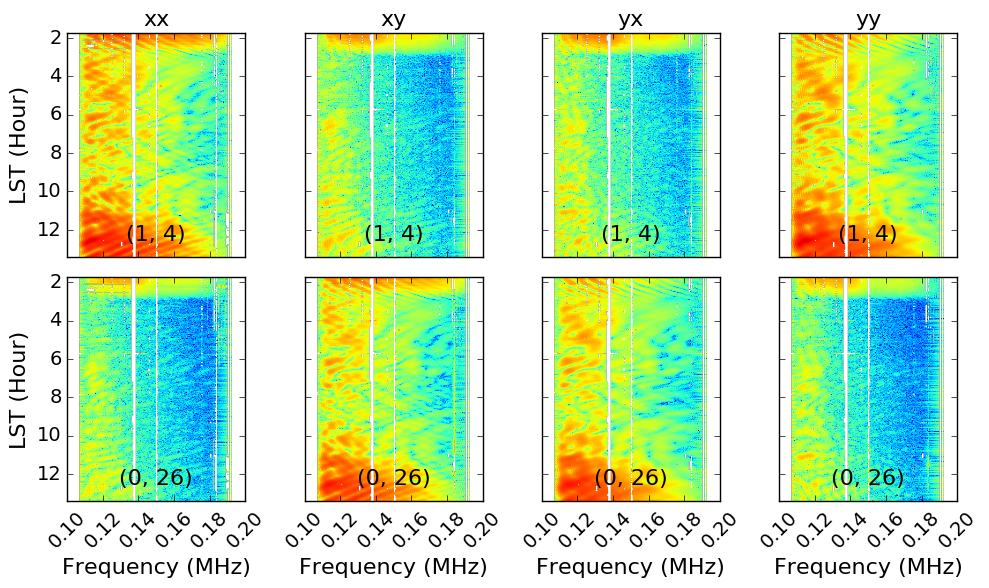
\includegraphics[width=0.96\textwidth]{plots/psa128_crosspol.png}
	\caption{Waterfall plots of visibility amplitudes for four different polarizations and two different baselines. Antenna 26 is found to be cross-polarized because its feed was rotated by 90 degrees, and hence its ``X" and ``Y" polarization states are mis-labeled. Equation \eqref{eq:psa128_crosspol} captures visibility amplitudes like the ones shown here in order to automatically detect cross-polarized antennae.}
	\label{fig:psa128_crosspol}
\end{figure}

Another failure mode is an antenna that exhibits low amplitude, a fairly common occurrence as different electronic components can cause the temporary reduction or loss of power. For example, low power can result from a malfunctioning amplifier or resistance somewhere along the signal chain. A particularly drastic example of power failure is when an entire correlator (FX2) was accidentally shut-off, cutting off connections to 16 antennas. The loss of those 16 antennas only affected Epoch 1, and the correlator was then re-started for Epoch 2. 

In order to find antennas with unusually low signals, we again employ Equation \eqref{eq:psa128_badant}, computing the metric for every antenna. Comparing $M_{i}$ across the entire array can reveal which antennas are consistently misbehaving. We then flag antennas with $M_{i}$ values that are low by at least $1\sigma$. Figure \ref{fig:psa128_badants} shows these antenna flags across both epochs, and we remove all data associated with antennas that are flagged greater than 50\% of the time (then for each epoch, we combine the flags for the XX and YY polarizations).

\begin{figure}
	\centering
	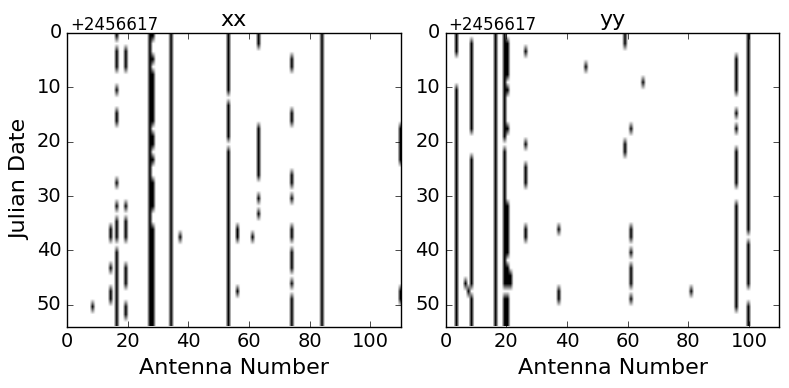
\includegraphics[trim={0cm 0cm 0cm 0cm},clip,height=0.35\textwidth]{plots/psa128_badants_S1E1.png}
	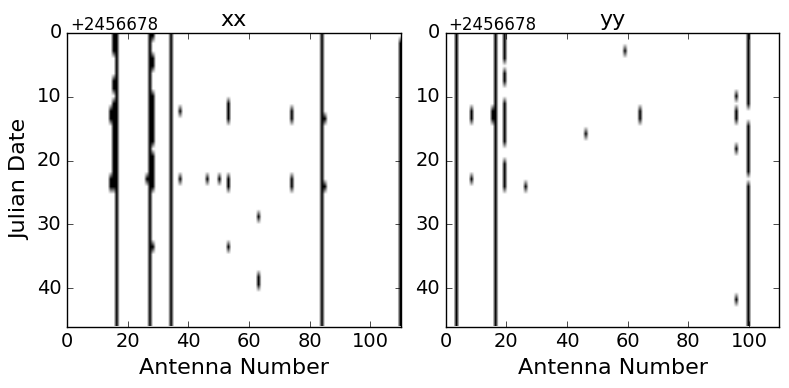
\includegraphics[trim={0cm 0cm 0cm 0cm},clip,height=0.35\textwidth]{plots/psa128_badants_S1E2.png}
	\caption{Flagged antennas, found using Equation \eqref{eq:psa128_badant}, are marked in black for each antenna number (x-axis) and Julian date (y-axis). The left column shows flags for XX polarization, and the right column shows flags for YY polarization. The top row shows flags for Epoch 1 and the bottom row shows flags for Epoch 2. We remove antennas that are flagged greater than 50\% of the time per epoch.}
	\label{fig:psa128_badants}
\end{figure}

Almost all of the flagged antennas listed in Table \ref{table:psa128_overview} are found via the metric described above. However, we do note that a handful are found manually by visually inspecting visibility data and {\tt Omnical} results. While our metric does a good job identifying antennas with low amplitudes, we found that there were certain antennas (usually one-off instances) with additional issues that do not fall under any of our previous metrics and would require a more sophisticated metric to be able to find automatically.

Finally, we highlight the importance of flagging antennas prior to redundant calibration by showing {\tt FirstCal} phase solutions for a single antenna without flagging and with flagging (Figure \ref{fig:psa128_chisq}, top). {\tt Omnical} $\chi^{2}$ results are also shown (bottom). These results depict how the quality of redundant calibration (the stability of the calibration solutions and level of redundancy) depends on the behavior of the antennas. It is evident that the {\tt FirstCal} solutions are unstable from file to file without any initial antenna flagging (top left). Similarly, higher $\chi^{2}$ values means that the {\tt Omnical} model visibilities differ substantially from the gain-corrected measured visibilities, meaning redundant calibration is poor. It is obvious that pre-calibration flagging metrics are crucial in order to robustly calibrate PAPER-128 data.

\begin{figure}
	\centering
	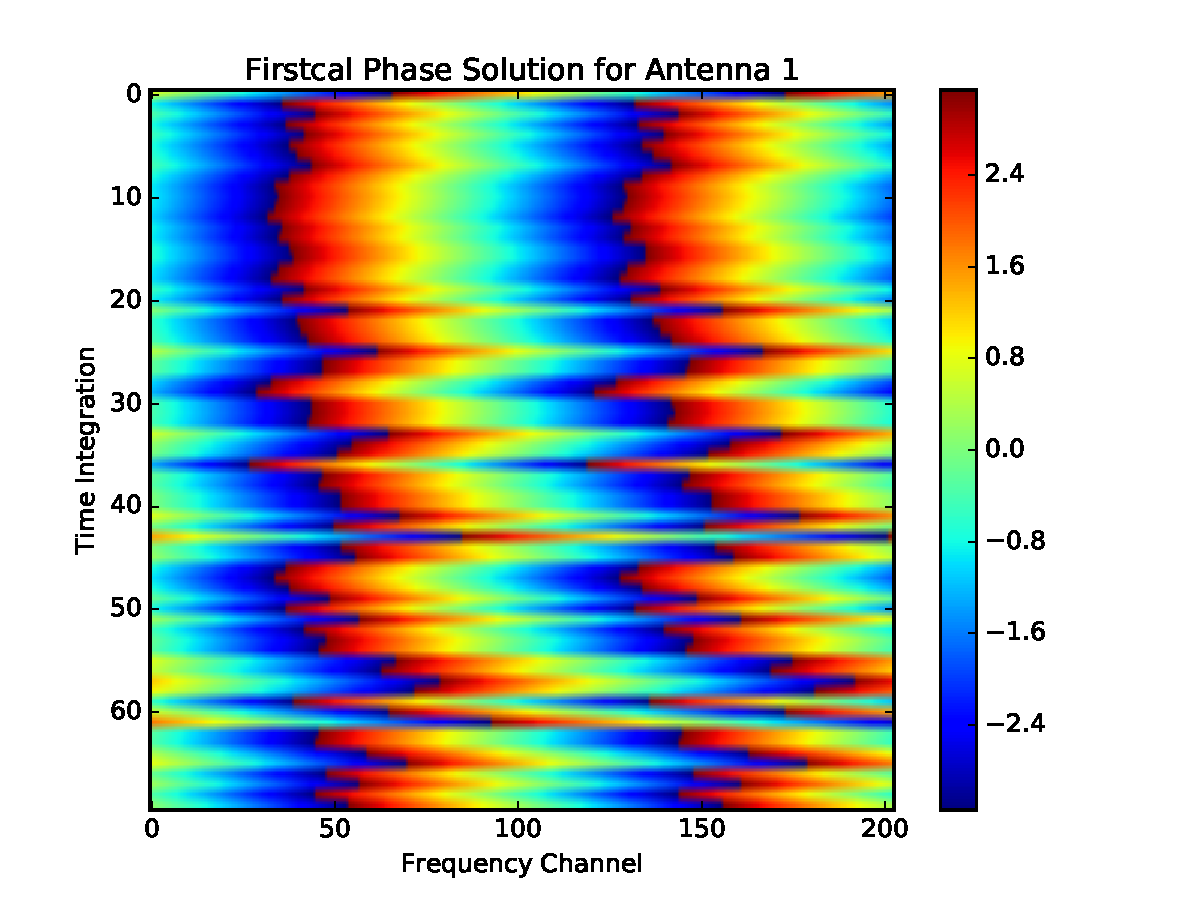
\includegraphics[trim={0cm 0cm 1cm 0cm},clip,height=0.35\textwidth]{plots/S1E1xx_nobadants_firstcal.pdf}
	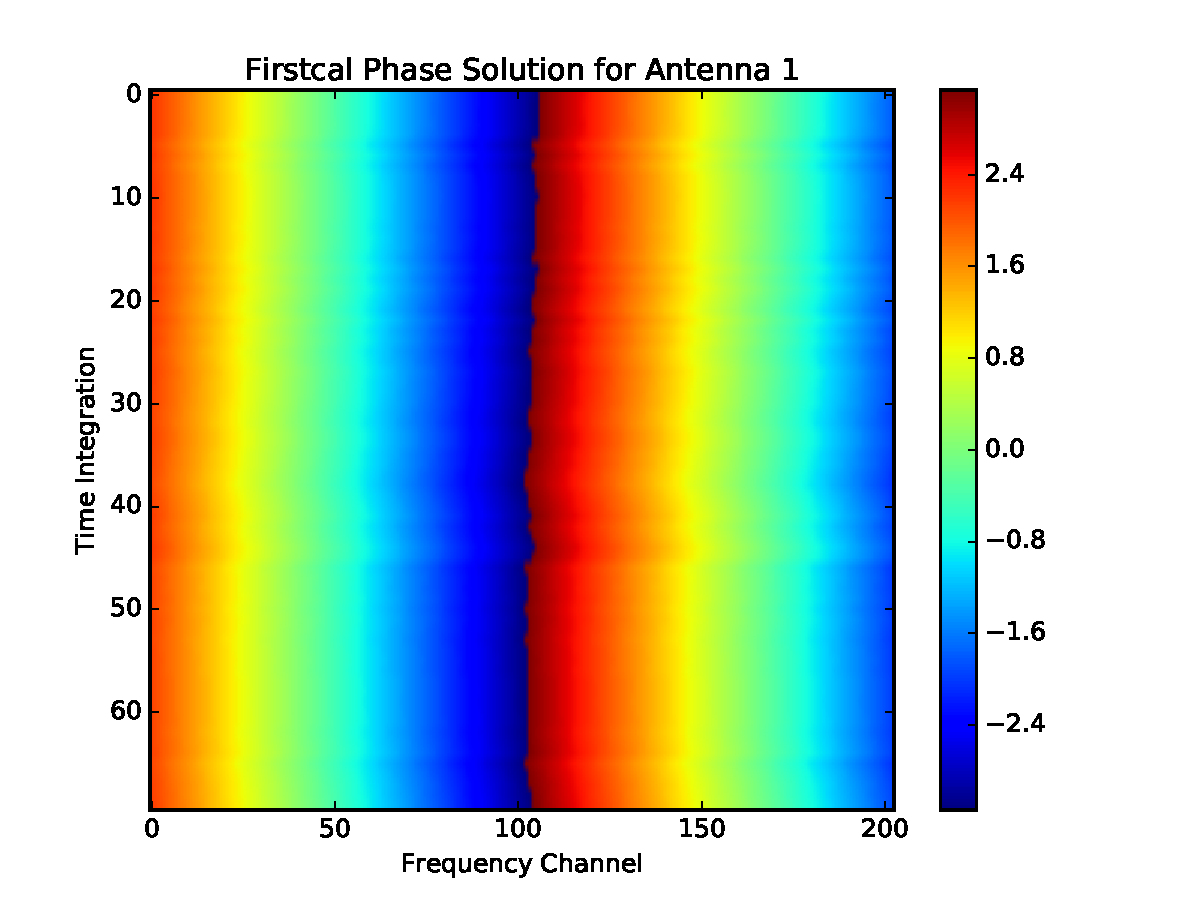
\includegraphics[trim={0cm 0cm 1cm 0cm},clip,height=0.35\textwidth]{plots/S1E1xx_withbadants_firstcal.pdf}
	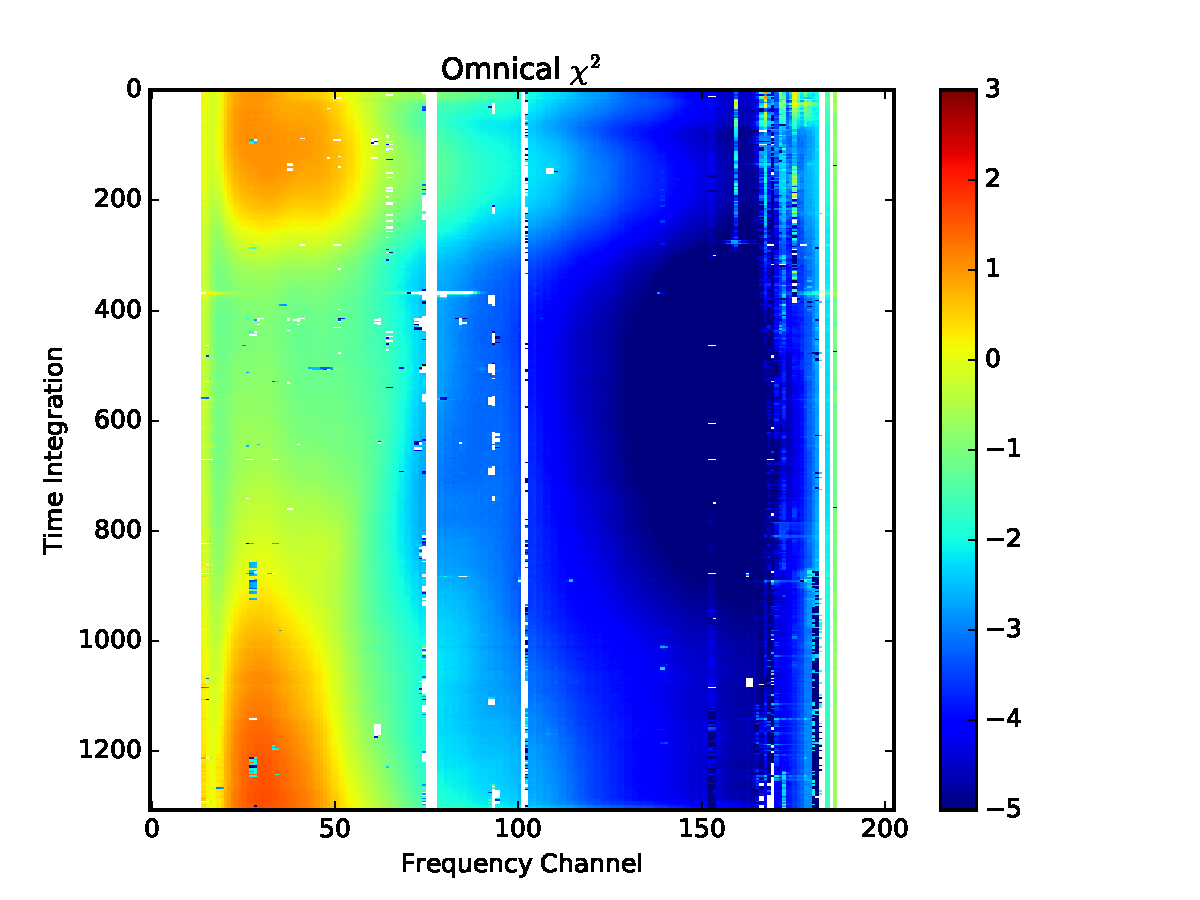
\includegraphics[trim={0cm 0cm 1cm 0cm},clip,height=0.35\textwidth]{plots/S1E1xx_nobadants_chisq.pdf}
	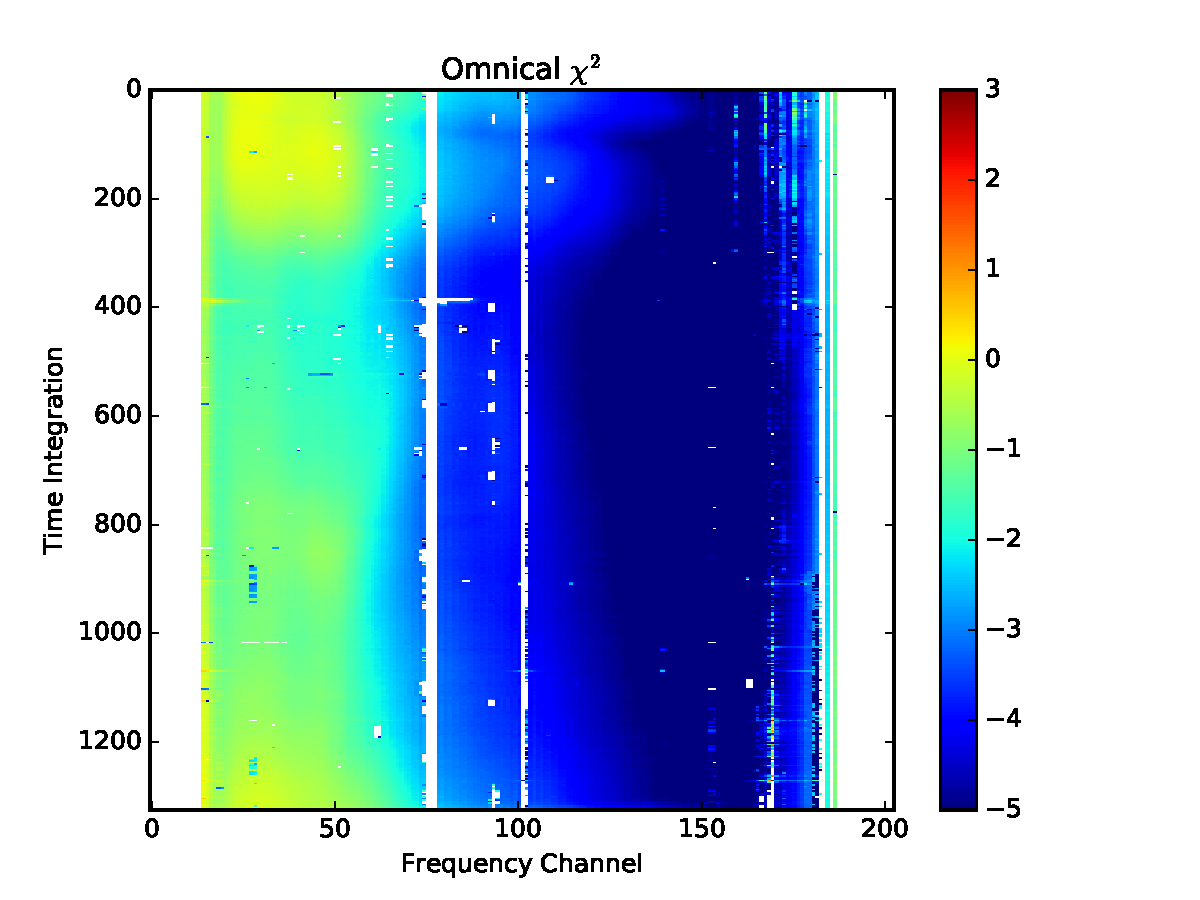
\includegraphics[trim={0cm 0cm 1cm 0cm},clip,height=0.35\textwidth]{plots/S1E1xx_withbadants_chisq.pdf}
	\caption{{\tt FirstCal} phase solutions for Antenna 1 (Epoch 1, XX polarization) where no antennas are flagged (top left) and some antennas are flagged (via the methods described in Chapter \ref{sec:psa128_badant}, top right). Omnical $\chi^{2}$ results are also shown for the two cases (bottom). We do not include any of the 16 dead antennas associated with correlator FX2. It is crucial to flag misbehaving antennas (especially extreme outlier antennas) prior to redundant calibration, motivating the development of automated quality assessment tools prior to the post-processing of data.}
	\label{fig:psa128_chisq}
\end{figure}

\section{Data Processing}

We process both epochs of PAPER-128 data, closely following the PAPER-64 processing steps outlined in Chapter \ref{sec:PSA64_processing}. One specific difference from the PAPER-64 pipeline is that we aggressively flag RFI prior to delay-filtering in order to prevent low levels of spectral structure from leaking into the EoR window. Because the overall quality of PAPER-128 data is in general lower than PAPER-64, we found that aggressive flagging methods are worthwhile in order to maximize signal-to-noise. To accomplish this, we first flag calibrated visibilities on a per-frequency, per-integration basis based on {\sc Omnical} $\chi^{2}$ values (using a $6\sigma$ deviation cutoff). This masks potentially problematic data identified from the redundant calibration solutions. In addition, we manually flag ten known channels containing RFI. 

Delay-filtering proceeds identically to the PAPER-64 pipeline. We then bin both the foreground-containing and foreground-removed data by LST into separate datasets. For both these datasets, we form Stokes I using Equation \eqref{eq:stokes}.

Recalling that redundant calibration only solves for internal calibration parameters, absolute calibration remains needed. In the PAPER-64 analysis, a self-calibration method was used to solve for overall gain and phase calibration solutions (immediately after redundant calibration) (\citealt{ali_et_al2015}). Trusting these solutions, we can then calibrate the PAPER-128 data to the calibrated PAPER-64 data. To do this, we use foreground-containing, LST-binned data for both PAPER-64 and PAPER-128 (where the PAPER-64 dataset is already calibrated) and look at a matching fiducial baseline for each. We align both datasets in LST and compute the ratio of the two for every time integration and frequency channel. We then average these ratios over time to yield a bandpass solution. 

Mathematically, if the visibility data for PAPER-64 and PAPER-128 are written as the following complex numbers:

\begin{eqnarray}
V_{64} = ae^{i\phi_{a}} \\
V_{128} = be^{i\phi_{b}},
\end{eqnarray}
we solve for an overall gain correction factor as:

\begin{equation}
f_{gain} = \frac{a}{b}
\end{equation}
and an overall phase factor as:

\begin{equation}
f_{\phi} = \phi_{a} - \phi_{b}.
\end{equation}
Combining these two gives a bandpass solution (one number per frequency):

\begin{equation}
f = f_{gain}e^{if_{\phi}}.
\end{equation}

Using this bandpass, we fit an eighth order polynomial to smooth the solutions and apply this multiplicative factor to the delay-filtered, LST-binned PAPER-64 data. We calibrate each epoch of data separately. We note that this coarse absolute calibration is only a rough calibration, and a more careful, sky-based calibration is recommended for precise results. However, using this simple calibration yields foreground data that agrees with the PAPER-64 data to within $\sim20\%$.

Finally, the last step of processing is fringe-rate filtering, where an optimal filter is used to combine the data and filter out excess noise. PAPER-128 has an original integration time of 32\,s, making the optimal filter length to be $\sim3910$\,s, slightly longer than that of PAPER-64. Armed with fringe-rate filtered, LST-binned datasets for both epochs, we proceed to power spectrum estimation.

\section{Power Spectrum Limits}

We form power spectrum estimates for both epochs of data and two frequency channel ranges: 139-149\,MHz (z=8.9) and 154-164\,MHz (z=7.9). Both bands consist of $21$ channels (each 0.5\,MHz) and are relatively absent of RFI. We focus only on one baseline-separation type, namely all 30\,m East/West baselines (of which there are 51 in the first epoch and 79 in the second). Our power spectrum formalism follows the analysis outlined in Chapter \ref{c.PSA64} and uses all updated methods regarding bootstrapping and noise sensitivity estimation. Because empirical inverse covariance weighting is shown to be extremely lossy for fringe-rate filtered PAPER data (Chapter \ref{sec:siglossmethod}) and regularization techniques do not significantly improve power spectrum sensitivity (Chapter \ref{sec:Weight}), we form unweighted limits ($\textbf{C} \equiv \textbf{I}$) in an effort to present straightforward, reliable results.

Figure \ref{fig:psa128_ps} shows the power spectrum results for PAPER-128. The two epochs are displayed as columns and the two redshifts as rows. Black and gray data points represent positive and negative power spectrum values, respectively (calculated as the average power spectrum value over all baseline pairs), and they have $2\sigma$ error bars that are calculated from bootstrapping over baselines. The solid green curve is our theoretical prediction of our sensitivity, computed analytically using Equation \eqref{eq:sense}. This sensitivity prediction is also plotted as gray shaded regions around the data points.

We note that our best limit is (126.4\,mK)$^{2}$ at $k = 0.29\,h$ Mpc$^{-1}$ and $z=7.9$ (from Epoch 2). This is a factor of XXX higher than our best limit from PAPER-64 (which uses three baselines instead of just one). These limits are understandably comparable given that the PAPER-128 analysis uses fewer days of data (by a factor of $\sim2$). While it's certainly possible that combining multiple epochs of data together (and using more baseline types) may yield better limits, we do not think this analysis is worthwhile as the second season of data is severely dominated by systematics. Instead, we look forward to exciting future results from HERA, knowing that many of the techniques developed for both PAPER-64 and PAPER-128 are being incorporated and improved upon.

\begin{figure}
	\centering
	\caption*{\hspace{0.6cm} Epoch 1 \hspace{5.6cm} Epoch 2}
	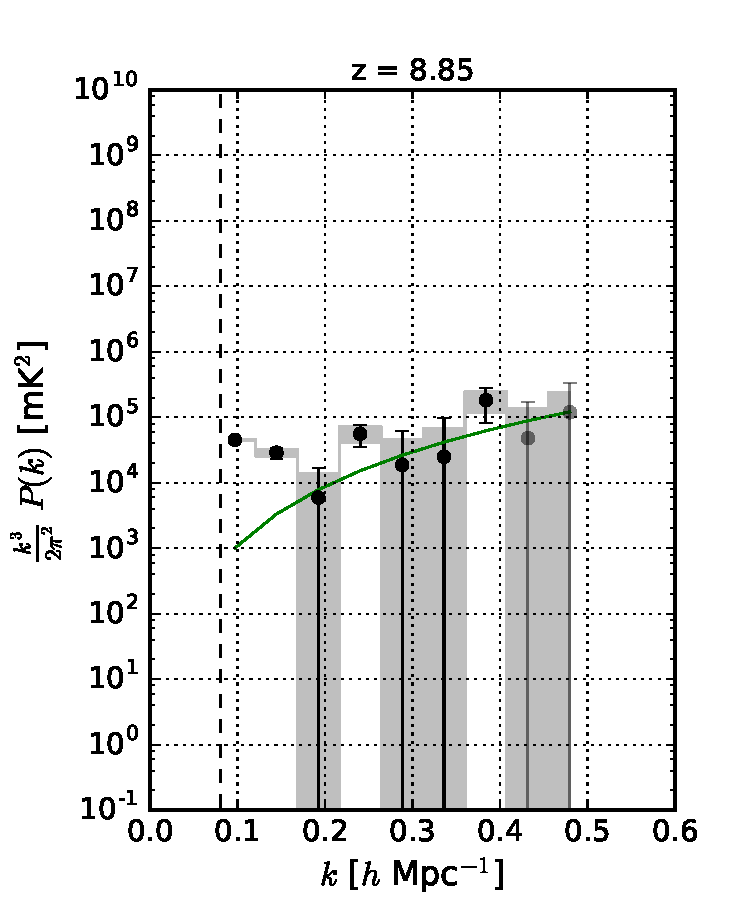
\includegraphics[trim={0cm 0cm 0cm 0.7cm},clip,height=0.5\textwidth]{plots/PSA128_S1E1_80_100.pdf}
	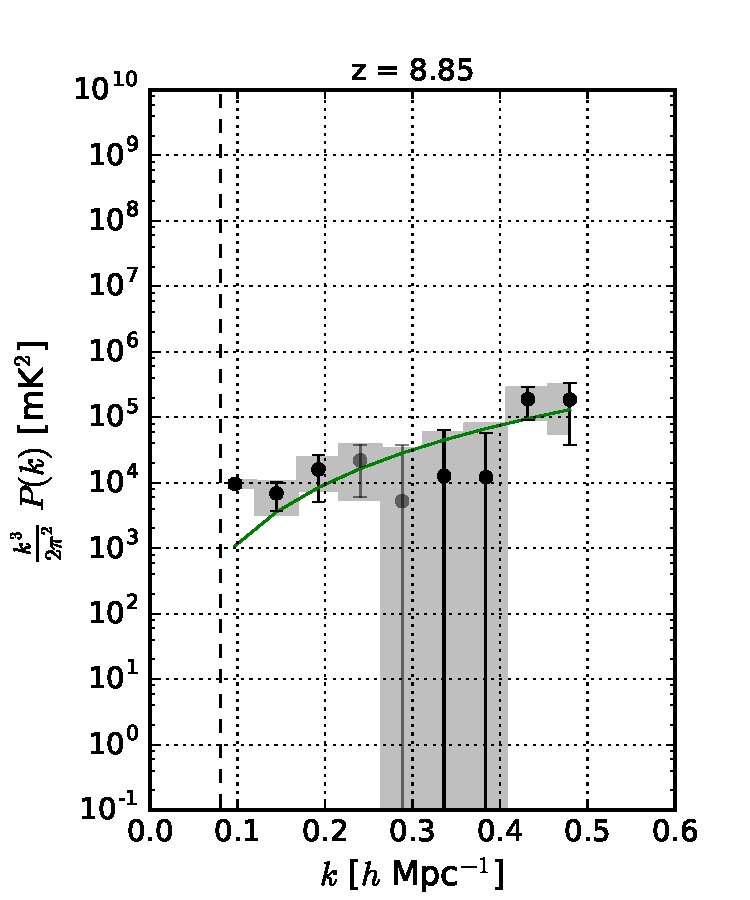
\includegraphics[trim={0cm 0cm 0cm 0.7cm},clip,height=0.5\textwidth]{plots/PSA128_S1E2_80_100.pdf}
	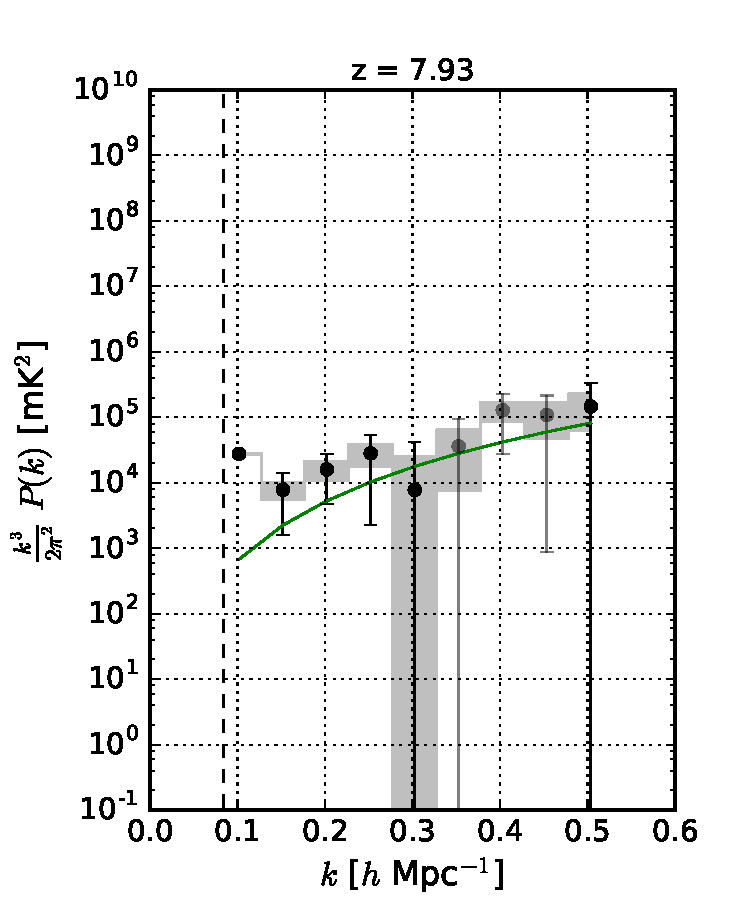
\includegraphics[trim={0cm 0cm 0cm 0.3cm},clip,height=0.5\textwidth]{plots/PSA128_S1E1_110_130.pdf}
	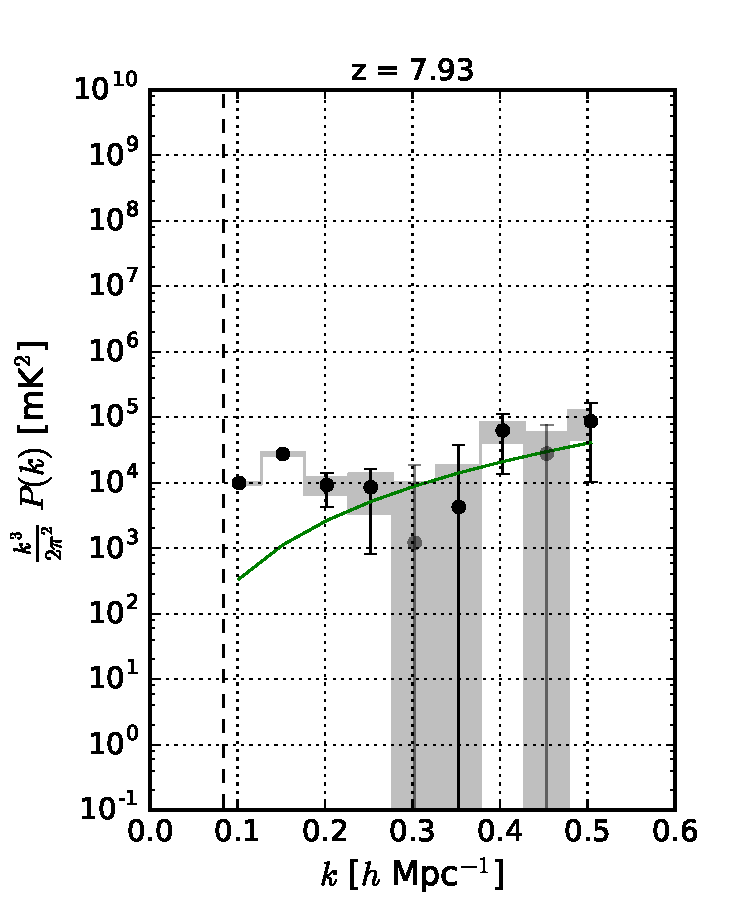
\includegraphics[trim={0cm 0cm 0cm 0.3cm},clip,height=0.5\textwidth]{plots/PSA128_S1E2_110_130.pdf}
	\caption*{\vspace{0.005cm}}
	\caption{Power spectrum results for PAPER-128 season 1 data for two redshifts (rows) and two epochs (columns), using one baseline separation-type only (30\,m East/West baselines). Black and gray points represent positive and negative power spectrum values, respectively, with $2\sigma$ error bars determined from bootstrapping. The $2\sigma$ theoretical noise sensitivity prediction is shown in green. Gray shaded regions correspond to theoretical errors on each data point.}
	\label{fig:psa128_ps}
\end{figure}
